\appendix
\renewcommand{\thesection}{APPENDIX \Alph{section}}
\section{ - Az izotóparány és az aktivitás számítása} \label{appendix:A}

\subsection{Az $^{235}$U -- $^{238}$U arány számítása}
Az $^{235}$U-höz tartozó magok részecskeszámának átlaga:

\begin{equation}
\overline{N}_{^{235}\text{U}}
=
\frac{5,74 + 8,18 + 9,21 + 9,03}{4} * 10^{18}
=
8,04 * 10^{18} \pm 5,97 * 10^{17}
\end{equation}
Míg az $^{238}$U-hoz tartozó magok részecskeszámának átlaga:

\begin{equation}
\overline{N}_{^{238}\text{U}}
=
\frac{1,94 * 10^{21} + 1,61 * 10^{21}}{2}
=
1,78 * 10^{21} \pm 9,82 * 10^{19}
\end{equation}
Ahol a hibákat az egyes izotópokhoz tartozó $N$ értékek relatív hibáinak négyzetes összege alapján számoltam. Ezek felhasználásával már megadhatóvá válnak az izotópok relatív koncentrációi:

\begin{equation}
C_{^{235}U}
=
\frac{8,04 * 10^{18}}{8,04 * 10^{18} + 1,78 * 10^{21}}
\approx
0.0045
=
0.45 \%
\end{equation}

\begin{equation}
C_{^{238}U}
=
\frac{1,78 * 10^{21}}{8,04 * 10^{18} + 1,78 * 10^{21}}
\approx
0.09955
=
99.55 \%
\end{equation}
A két arány relatív hibája megegyezik a $N$ relatív hibájával, így a hibával ellátott végeredmény:

\begin{equation}
C_{^{235}U}
=
0,0045 \pm 0,0003
=
\left( 0,45 \pm 0,03 \right) \%
\end{equation}

\begin{equation}
C_{^{238}U}
=
0,9955 \pm 0,0550
=
\left( 99,55 \pm 5,50 \right) \%
\end{equation}
Ahol a két koncentráció relatív hibáját az egyes izotópokhoz tartozó $N$ részecskeszámok relatív hibáinak négyzetes összege adta.

\subsection{A súlyozott átlag számítása}
A minta teljes súlyozott aktivitása megkapható az alábbi számításból, felhasználva a \ref{table:4}. táblázatban található értékeket:
\begin{align}
\left< A \right>
&=
\dfrac{
\dfrac{179,1\ \text{Bq}}{\left( 5,8\ \text{Bq} \right)^{2}}
+
\dfrac{255,2\ \text{Bq}}{\left( 11,9\ \text{Bq} \right)^{2}}
+
\dfrac{287,4\ \text{Bq}}{\left( 6,5\ \text{Bq} \right)^{2}}
+
\dfrac{281,8\ \text{Bq}}{\left( 11,9\ \text{Bq} \right)^{2}}
+
\dfrac{9554,6\ \text{Bq}}{\left( 430,1\ \text{Bq} \right)^{2}}
+
\dfrac{7939,6\ \text{Bq}}{\left( 254,3\ \text{Bq} \right)^{2}}
}{
\dfrac{1}{\left( 5,8\ \text{Bq} \right)^{2}}
+
\dfrac{1}{\left( 11,9\ \text{Bq} \right)^{2}}
+
\dfrac{1}{\left( 6,5\ \text{Bq} \right)^{2}}
+
\dfrac{1}{\left( 11,9\ \text{Bq} \right)^{2}}
+
\dfrac{1}{\left( 430,1\ \text{Bq} \right)^{2}}
+
\dfrac{1}{\left( 254,3\ \text{Bq} \right)^{2}}
}
= \nonumber \\
&=
\dfrac{16,189\ \dfrac{1}{\text{Bq}}}{0,067\ \dfrac{1}{\text{Bq}^{2}}}
=
238,34\ \text{Bq}
\end{align}
Ennek hibája megadható a következő módon:

\begin{align}
\sigma_{\left< A \right>}
&=
\dfrac{1}{\sqrt{
\dfrac{1}{\left( 5,8\ \text{Bq} \right)^{2}}
+
\dfrac{1}{\left( 11,9\ \text{Bq} \right)^{2}}
+
\dfrac{1}{\left( 6,5\ \text{Bq} \right)^{2}}
+
\dfrac{1}{\left( 11,9\ \text{Bq} \right)^{2}}
+
\dfrac{1}{\left( 430,1\ \text{Bq} \right)^{2}}
+
\dfrac{1}{\left( 254,3\ \text{Bq} \right)^{2}}
}}
= \nonumber \\
&=
\dfrac{1}{\sqrt{0,067\ \dfrac{1}{\text{Bq}^{2}}}}
=
3,84\ \text{Bq}
\end{align}
\newpage
\section{ - Ábrák} \label{appendix:B}
\topskip0pt
\vspace*{\fill}
\begin{center}
    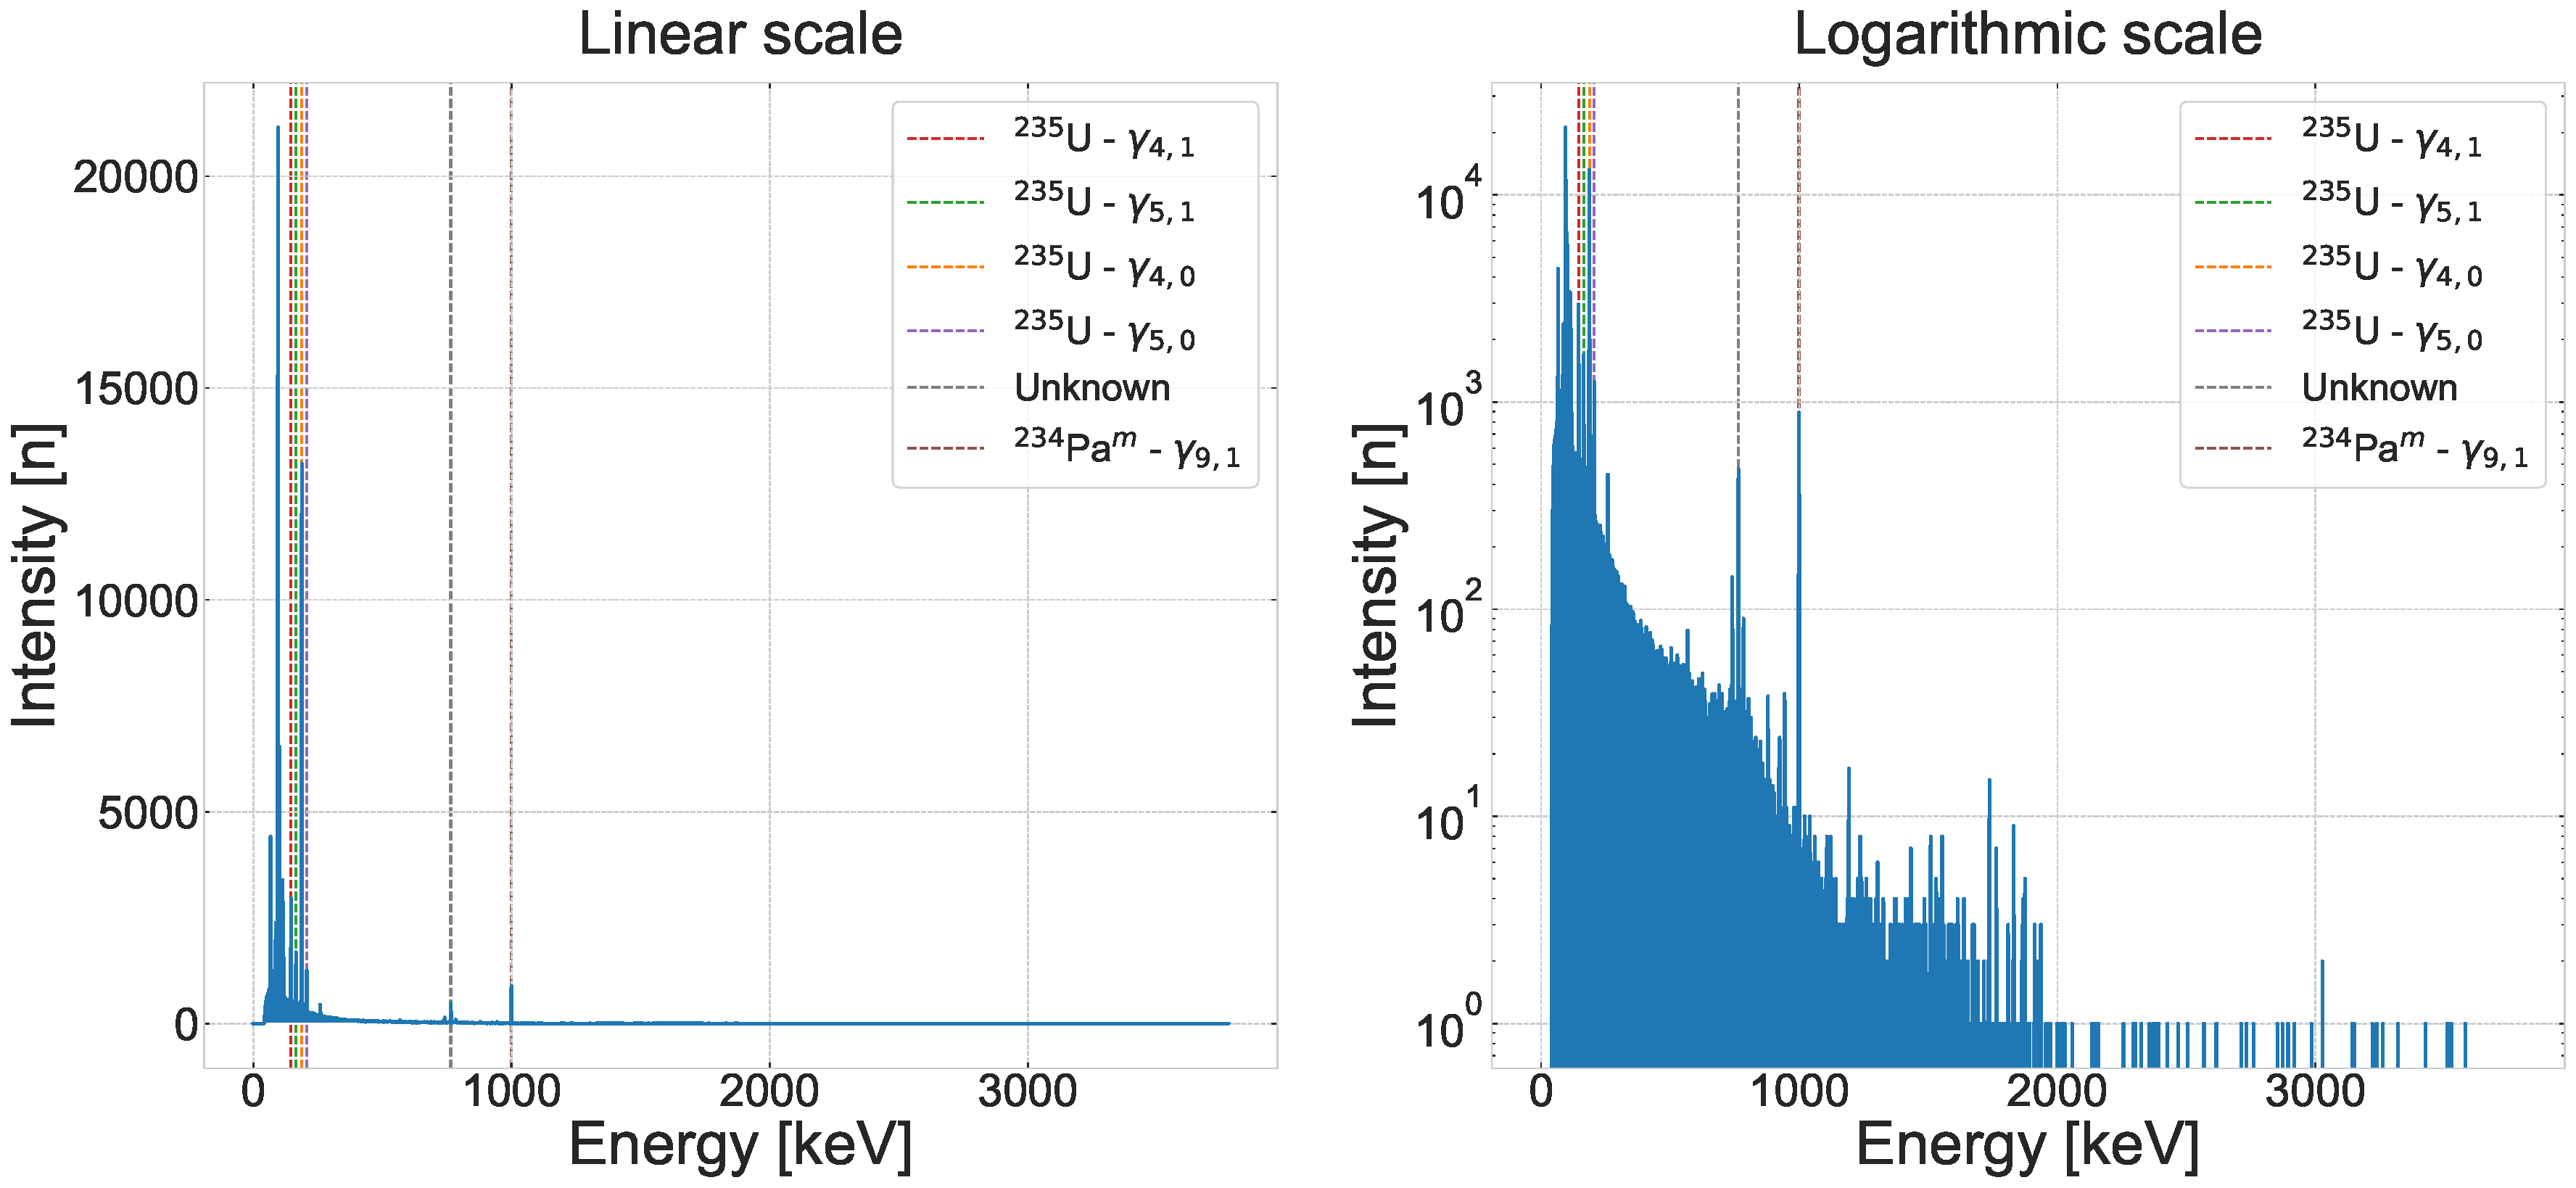
\includegraphics[width=\textwidth]{{images/full_spectra}.pdf}
    \captionof{figure}{Az általam vizsgált anyag teljes lemért gamma-spektruma. Az egyes karakterisztikus csúcsok színes, szaggatott vonallal vannak jelölve.} \label{fig:1}
\end{center}
\begin{center}
    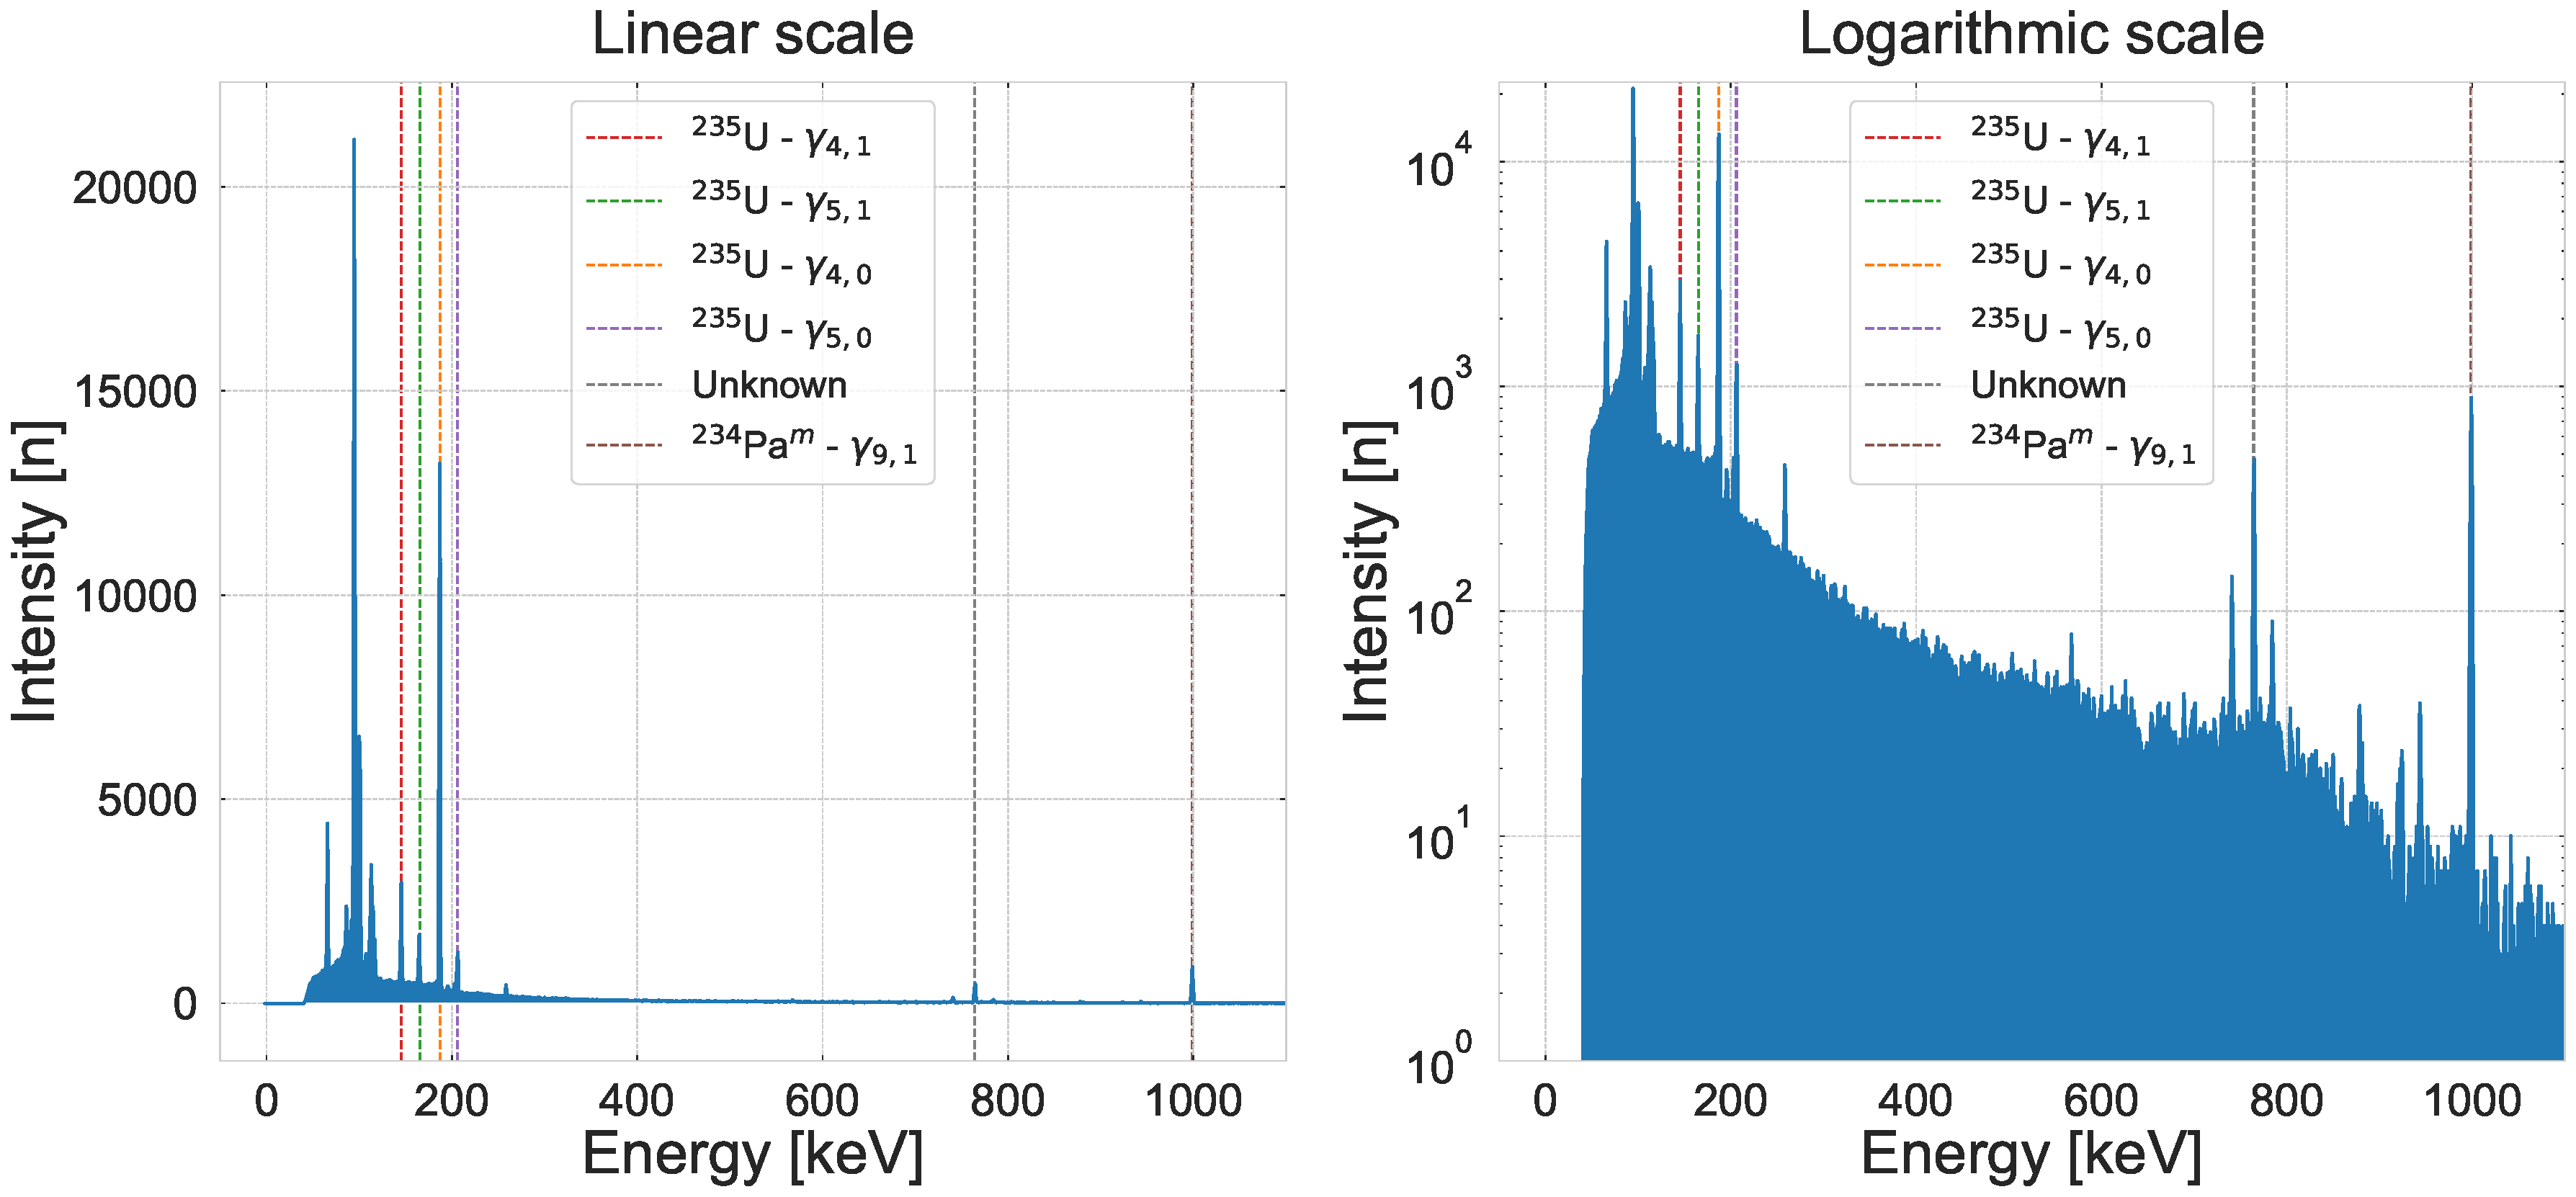
\includegraphics[width=\textwidth]{{images/spectra_lims_-50.00_1100.00_full_height}.pdf}
    \captionof{figure}{Az általam vizsgált anyag gamma-spektruma a $0\ \text{keV} - 1100\ \text{keV}$ intervallumban. Az egyes karakterisztikus csúcsok színes, szaggatott vonallal vannak jelölve.} \label{fig:2}
\end{center}
\begin{center}
    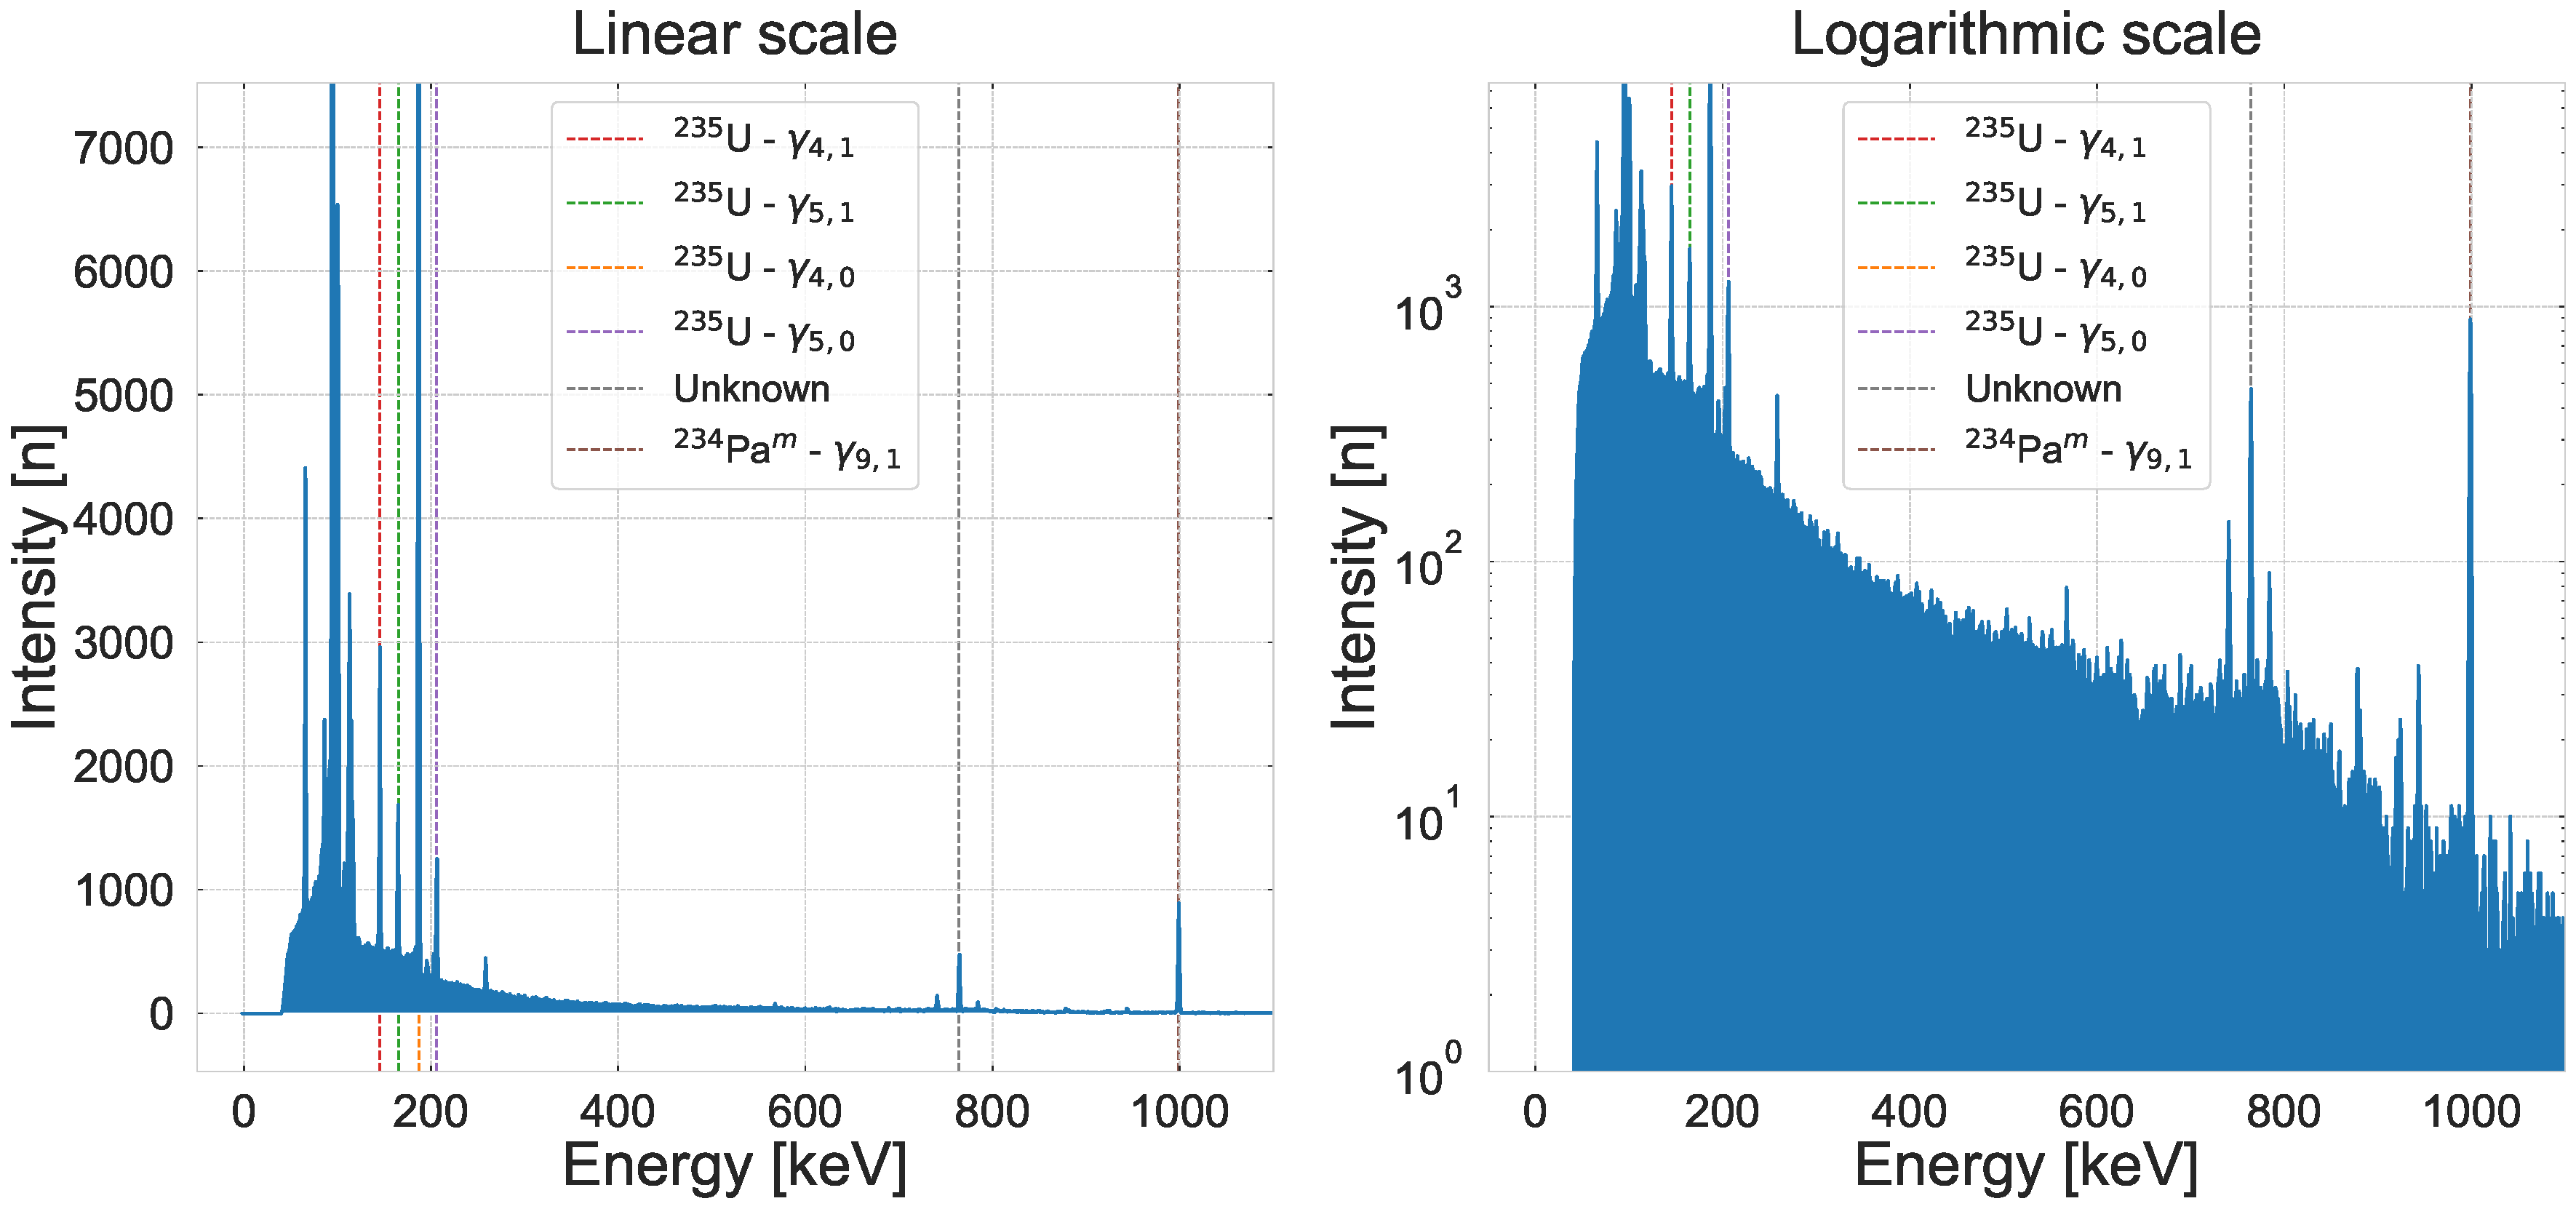
\includegraphics[width=\textwidth]{{images/spectra_lims_-50.00_1100.00_small_height}.pdf}
    \captionof{figure}{Az általam vizsgált anyag gamma-spektruma a $0\ \text{keV} - 1100\ \text{keV}$ intervallumban. Az ábrán a (\ref{fig:2})-es ábrán szereplő $y$-tengely alsó harmada van megjelenítve. Az egyes karakterisztikus csúcsok színes, szaggatott vonallal vannak jelölve.} \label{fig:3}
\end{center}
\vspace*{\fill}
\newpage
\topskip0pt
\vspace*{\fill}
\begin{center}
    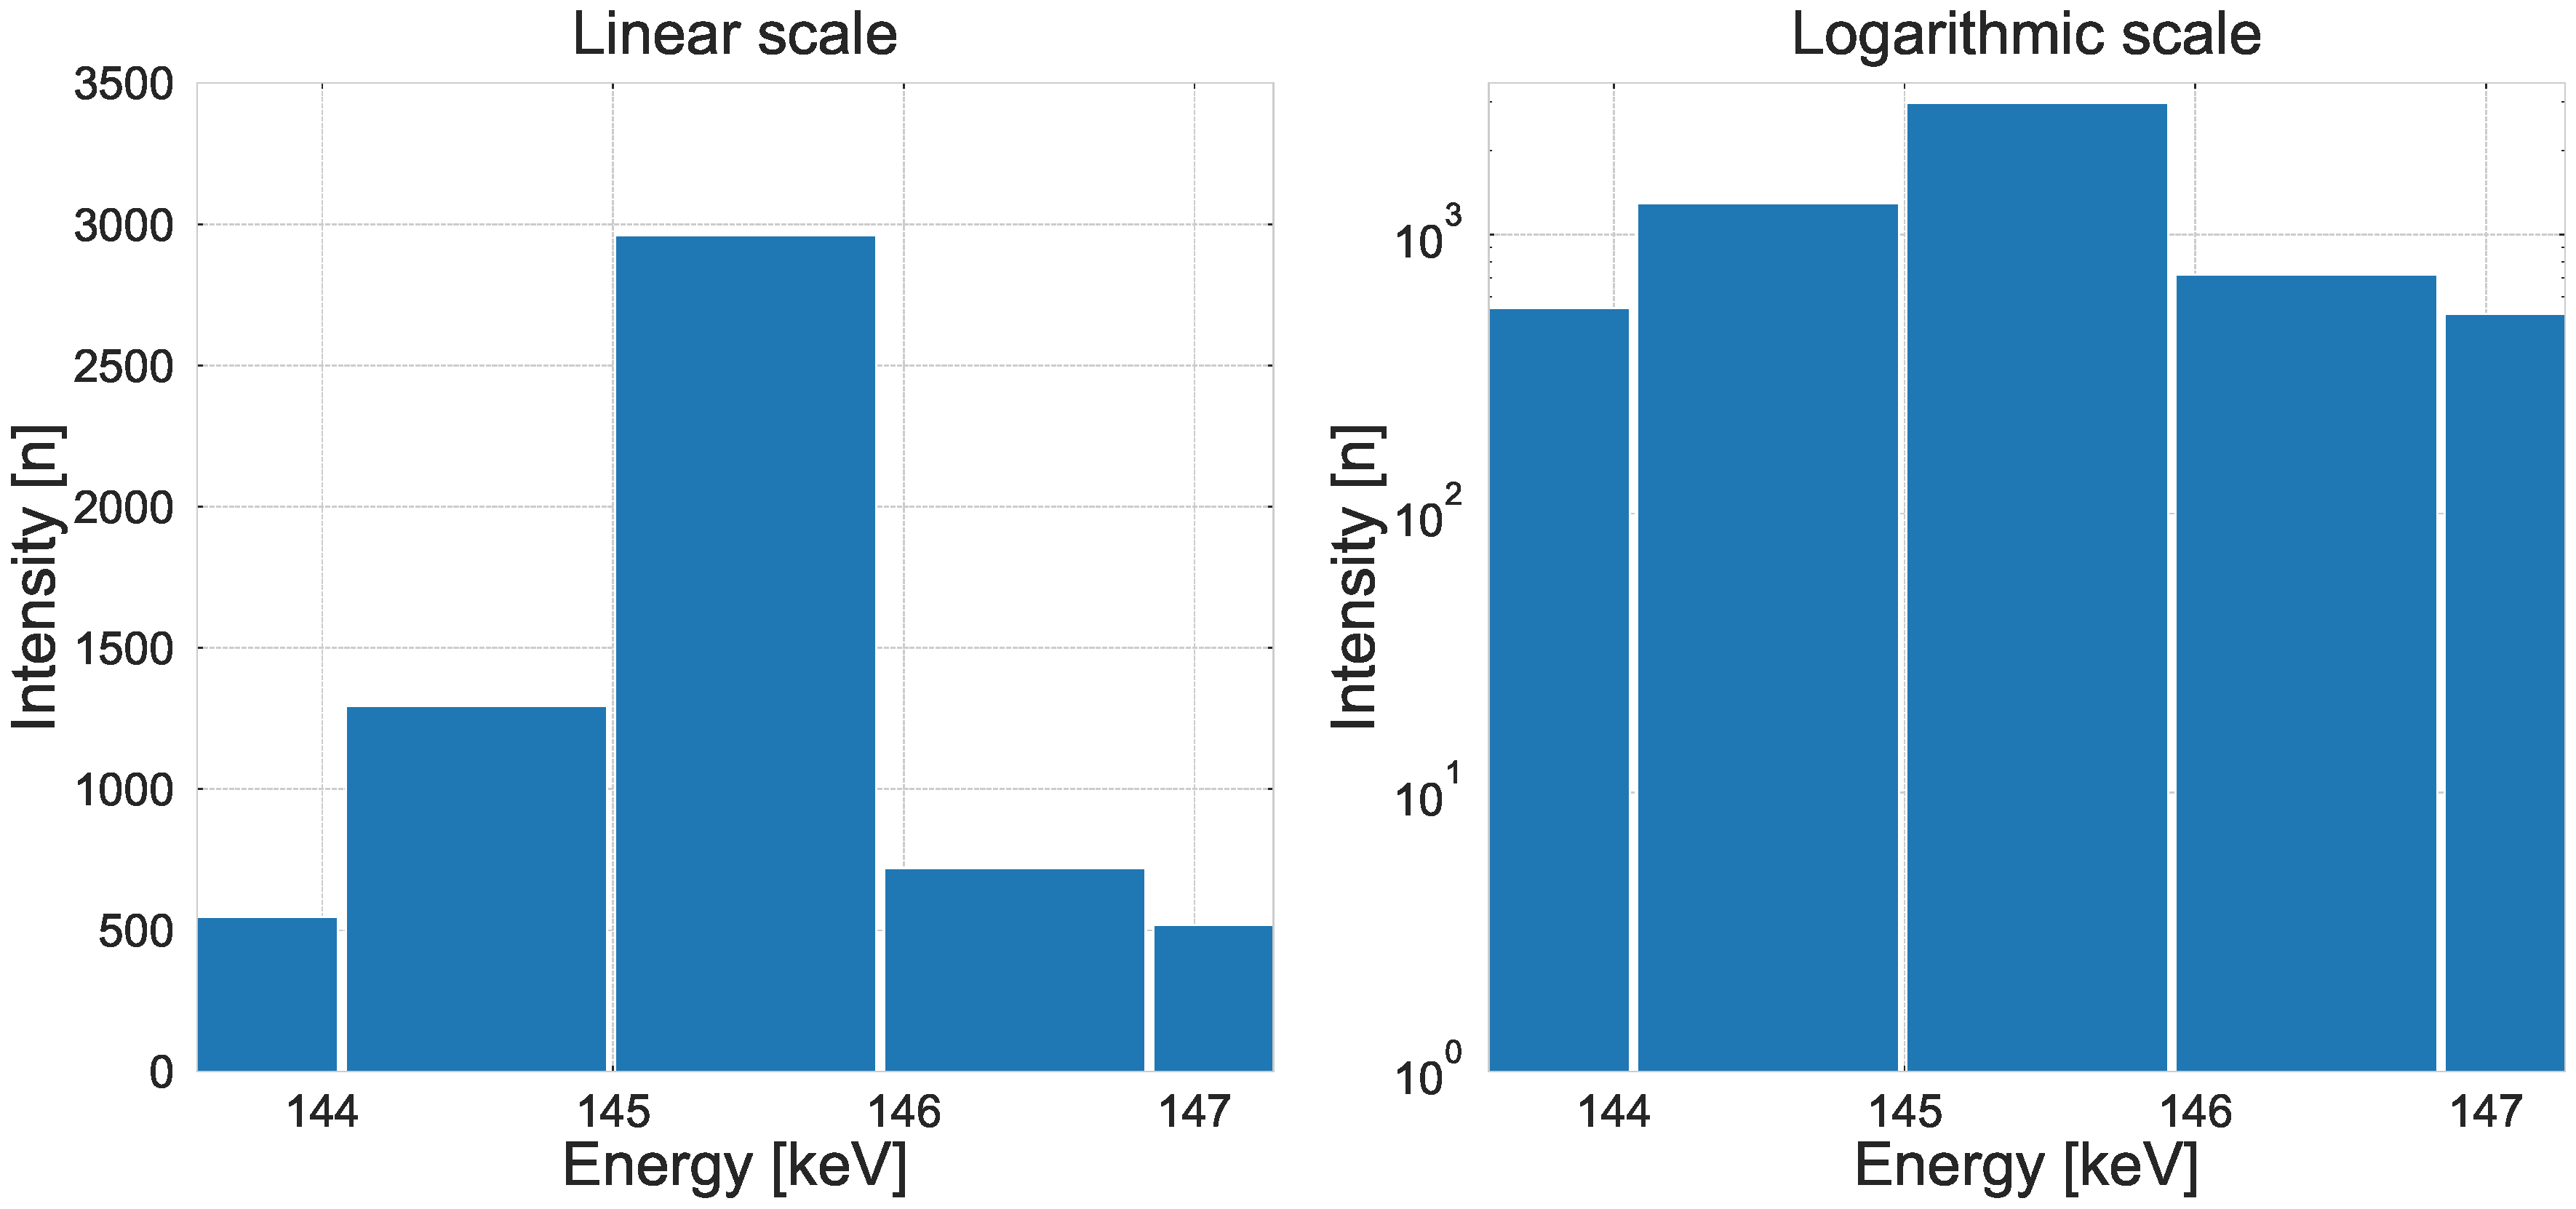
\includegraphics[width=\textwidth]{{images/spectra_lims_143.57_147.27_U235_g4_1}.pdf}
    \captionof{figure}{Az általam vizsgált anyag gamma-spektrumában található $^{235}$U, $\gamma_{4,1}$ tranziensből származó fotonjának foto-csúcsa.} \label{fig:4}
\end{center}
\begin{center}
    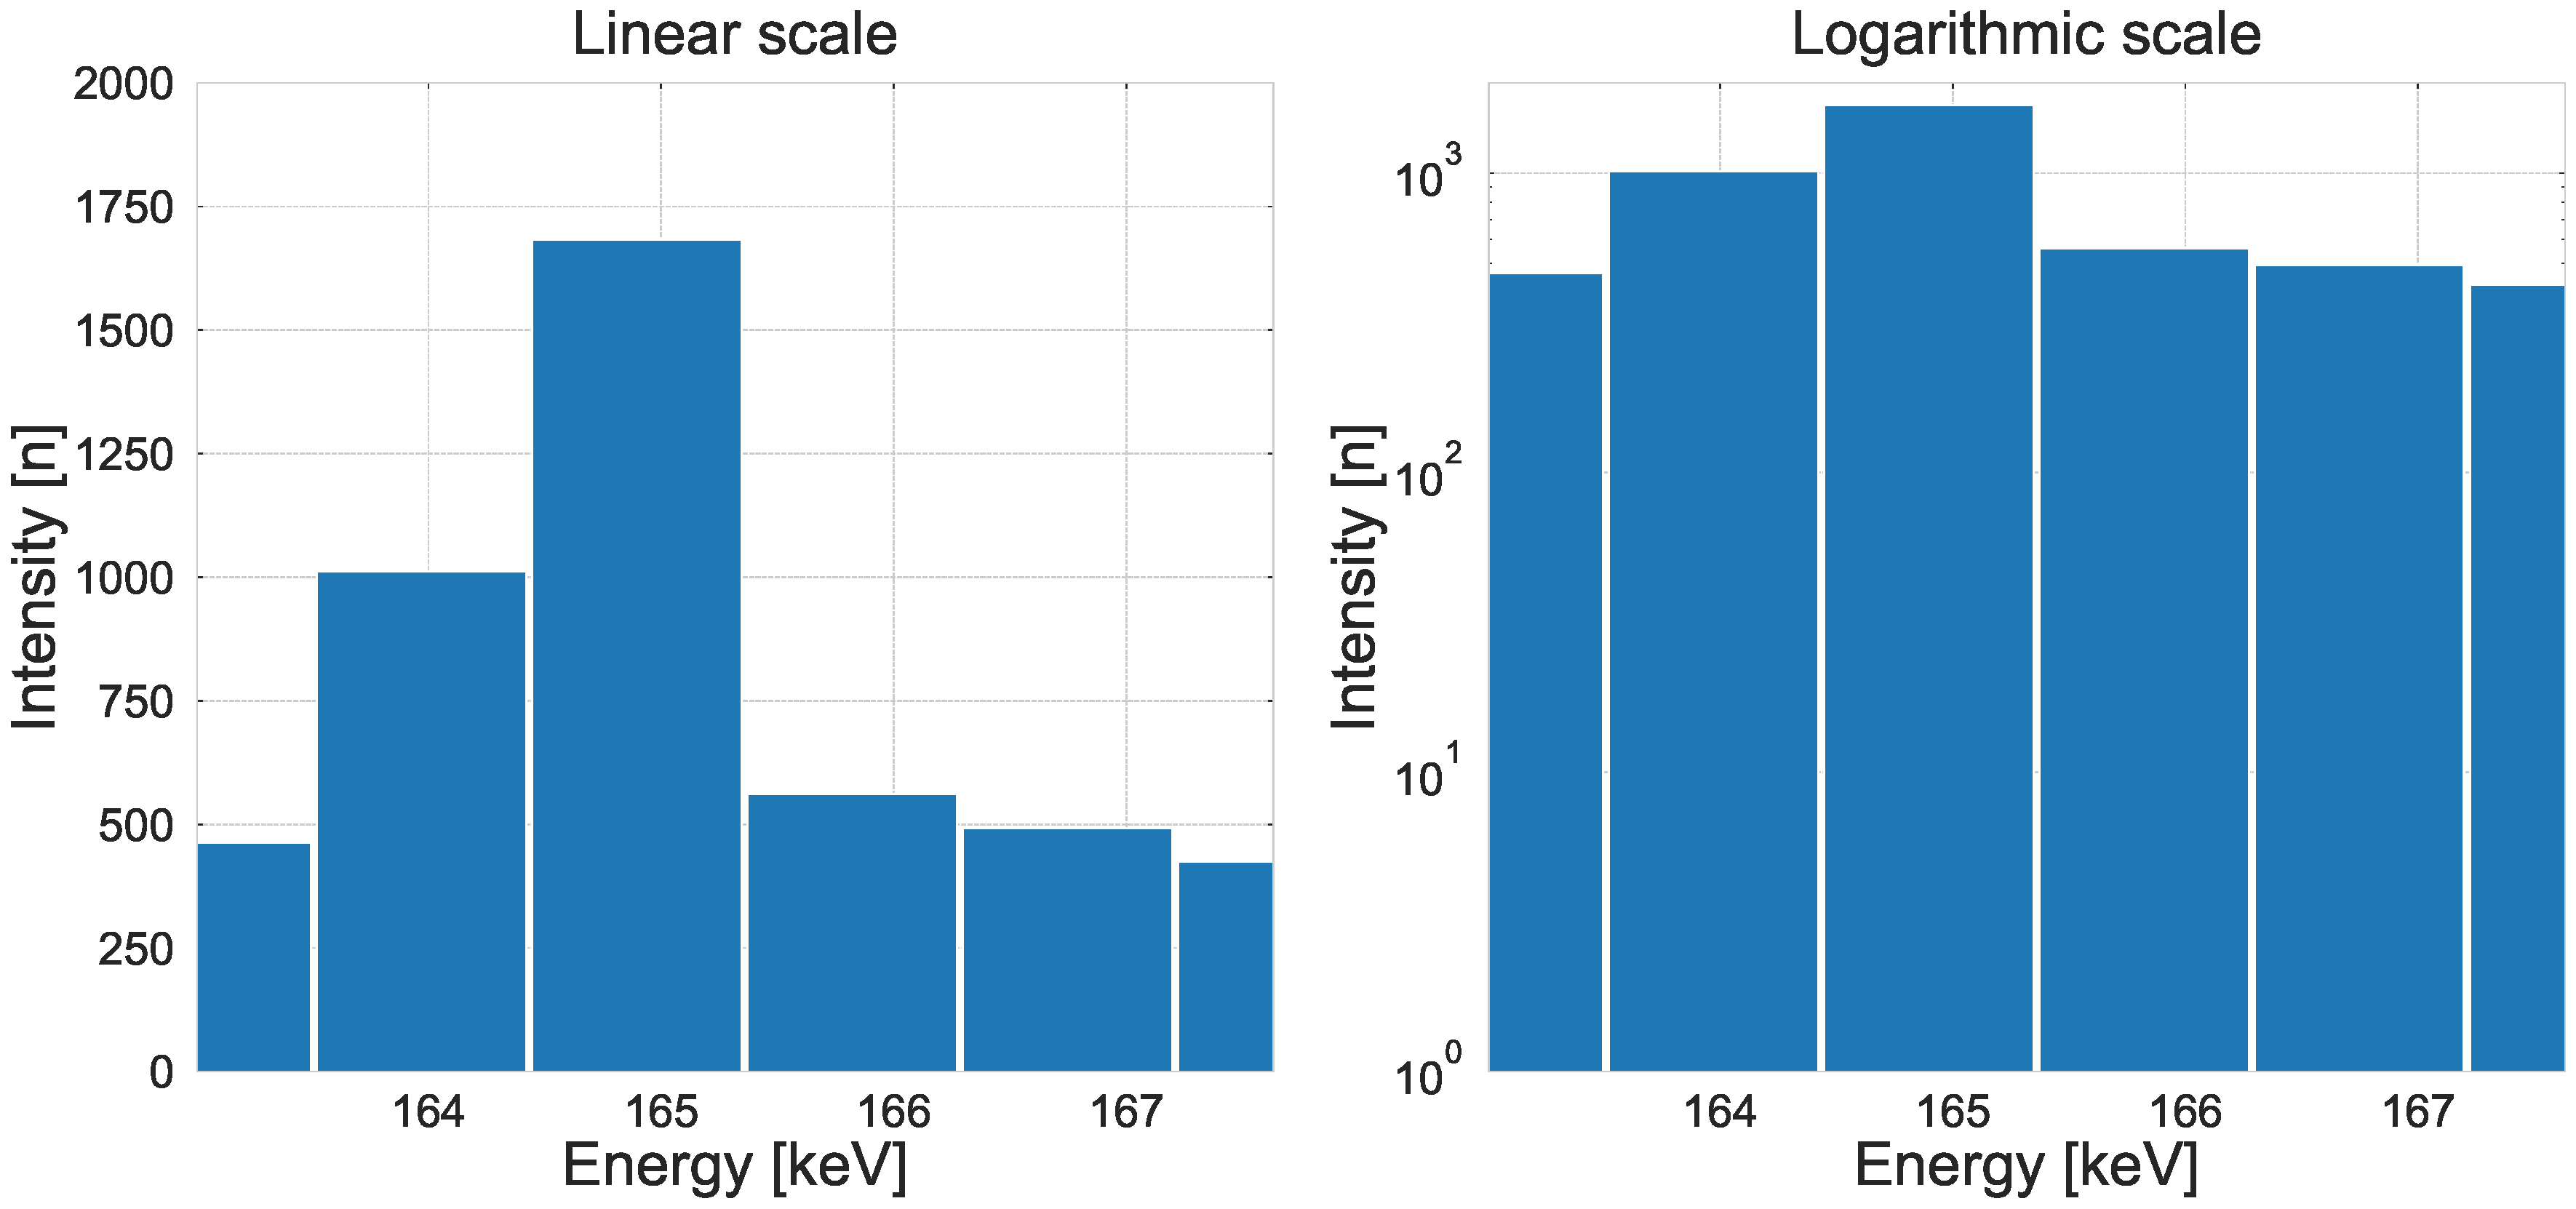
\includegraphics[width=\textwidth]{{images/spectra_lims_163.00_167.63_U235_g5_1}.pdf}
    \captionof{figure}{Az általam vizsgált anyag gamma-spektrumában található $^{235}$U, $\gamma_{5,1}$ tranziensből származó fotonjának foto-csúcsa.} \label{fig:5}
\end{center}
\begin{center}
    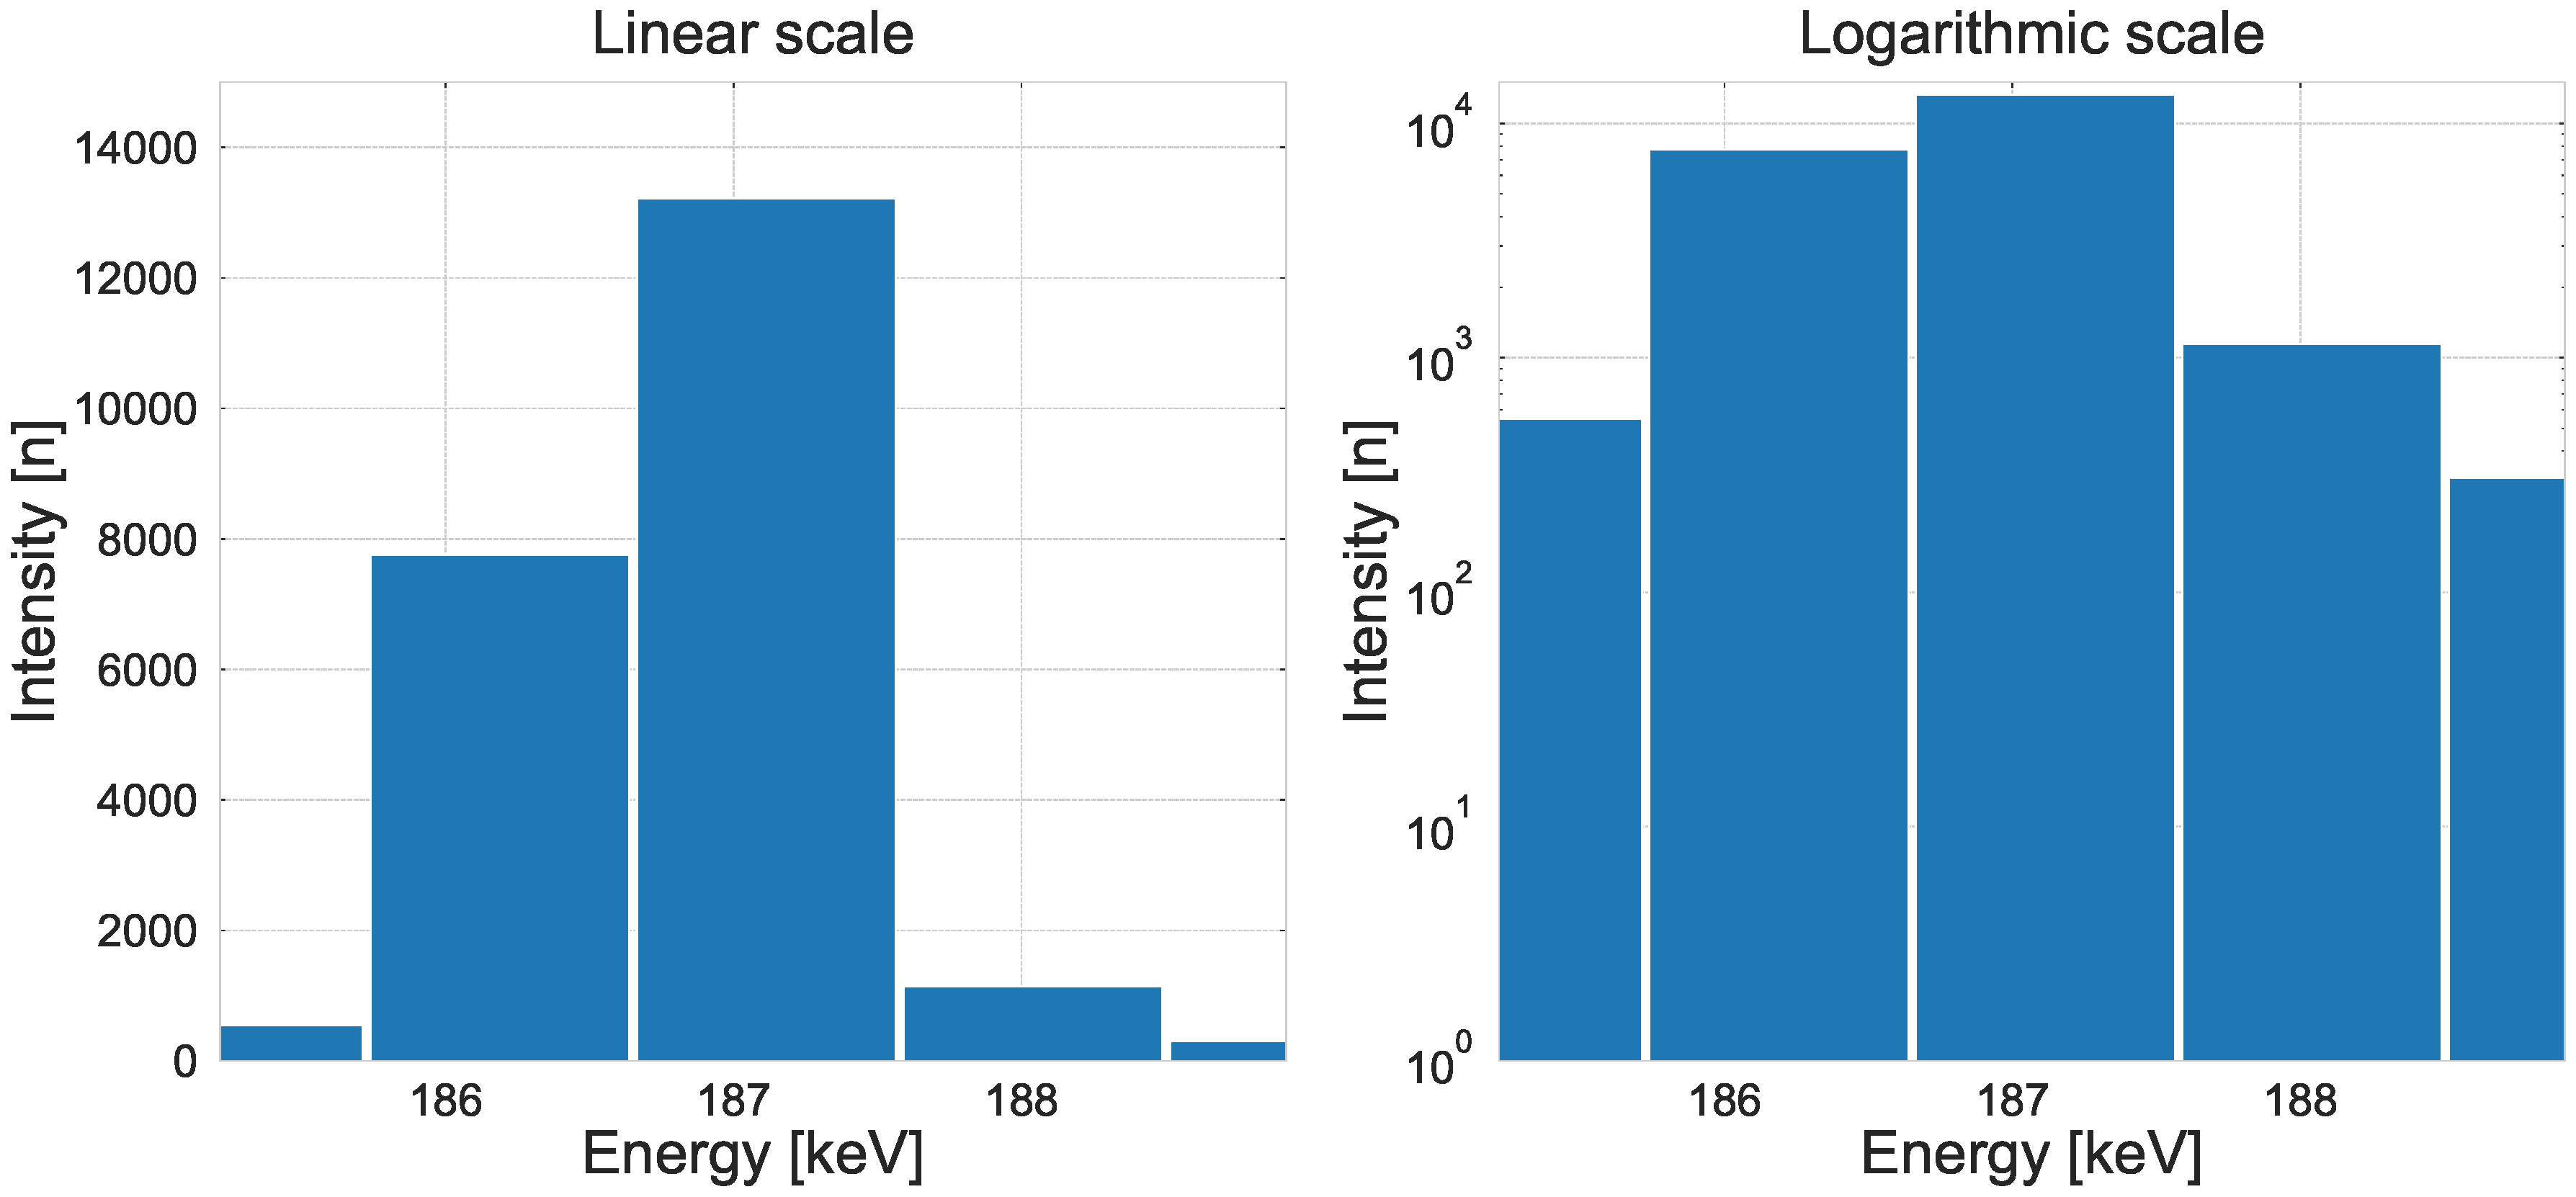
\includegraphics[width=\textwidth]{{images/spectra_lims_185.22_188.92_U235_g4_0}.pdf}
    \captionof{figure}{Az általam vizsgált anyag gamma-spektrumában található $^{235}$U, $\gamma_{4,0}$ tranziensből származó fotonjának foto-csúcsa.} \label{fig:6}
\end{center}
\vspace*{\fill}
\newpage
\topskip0pt
\vspace*{\fill}
\begin{center}
    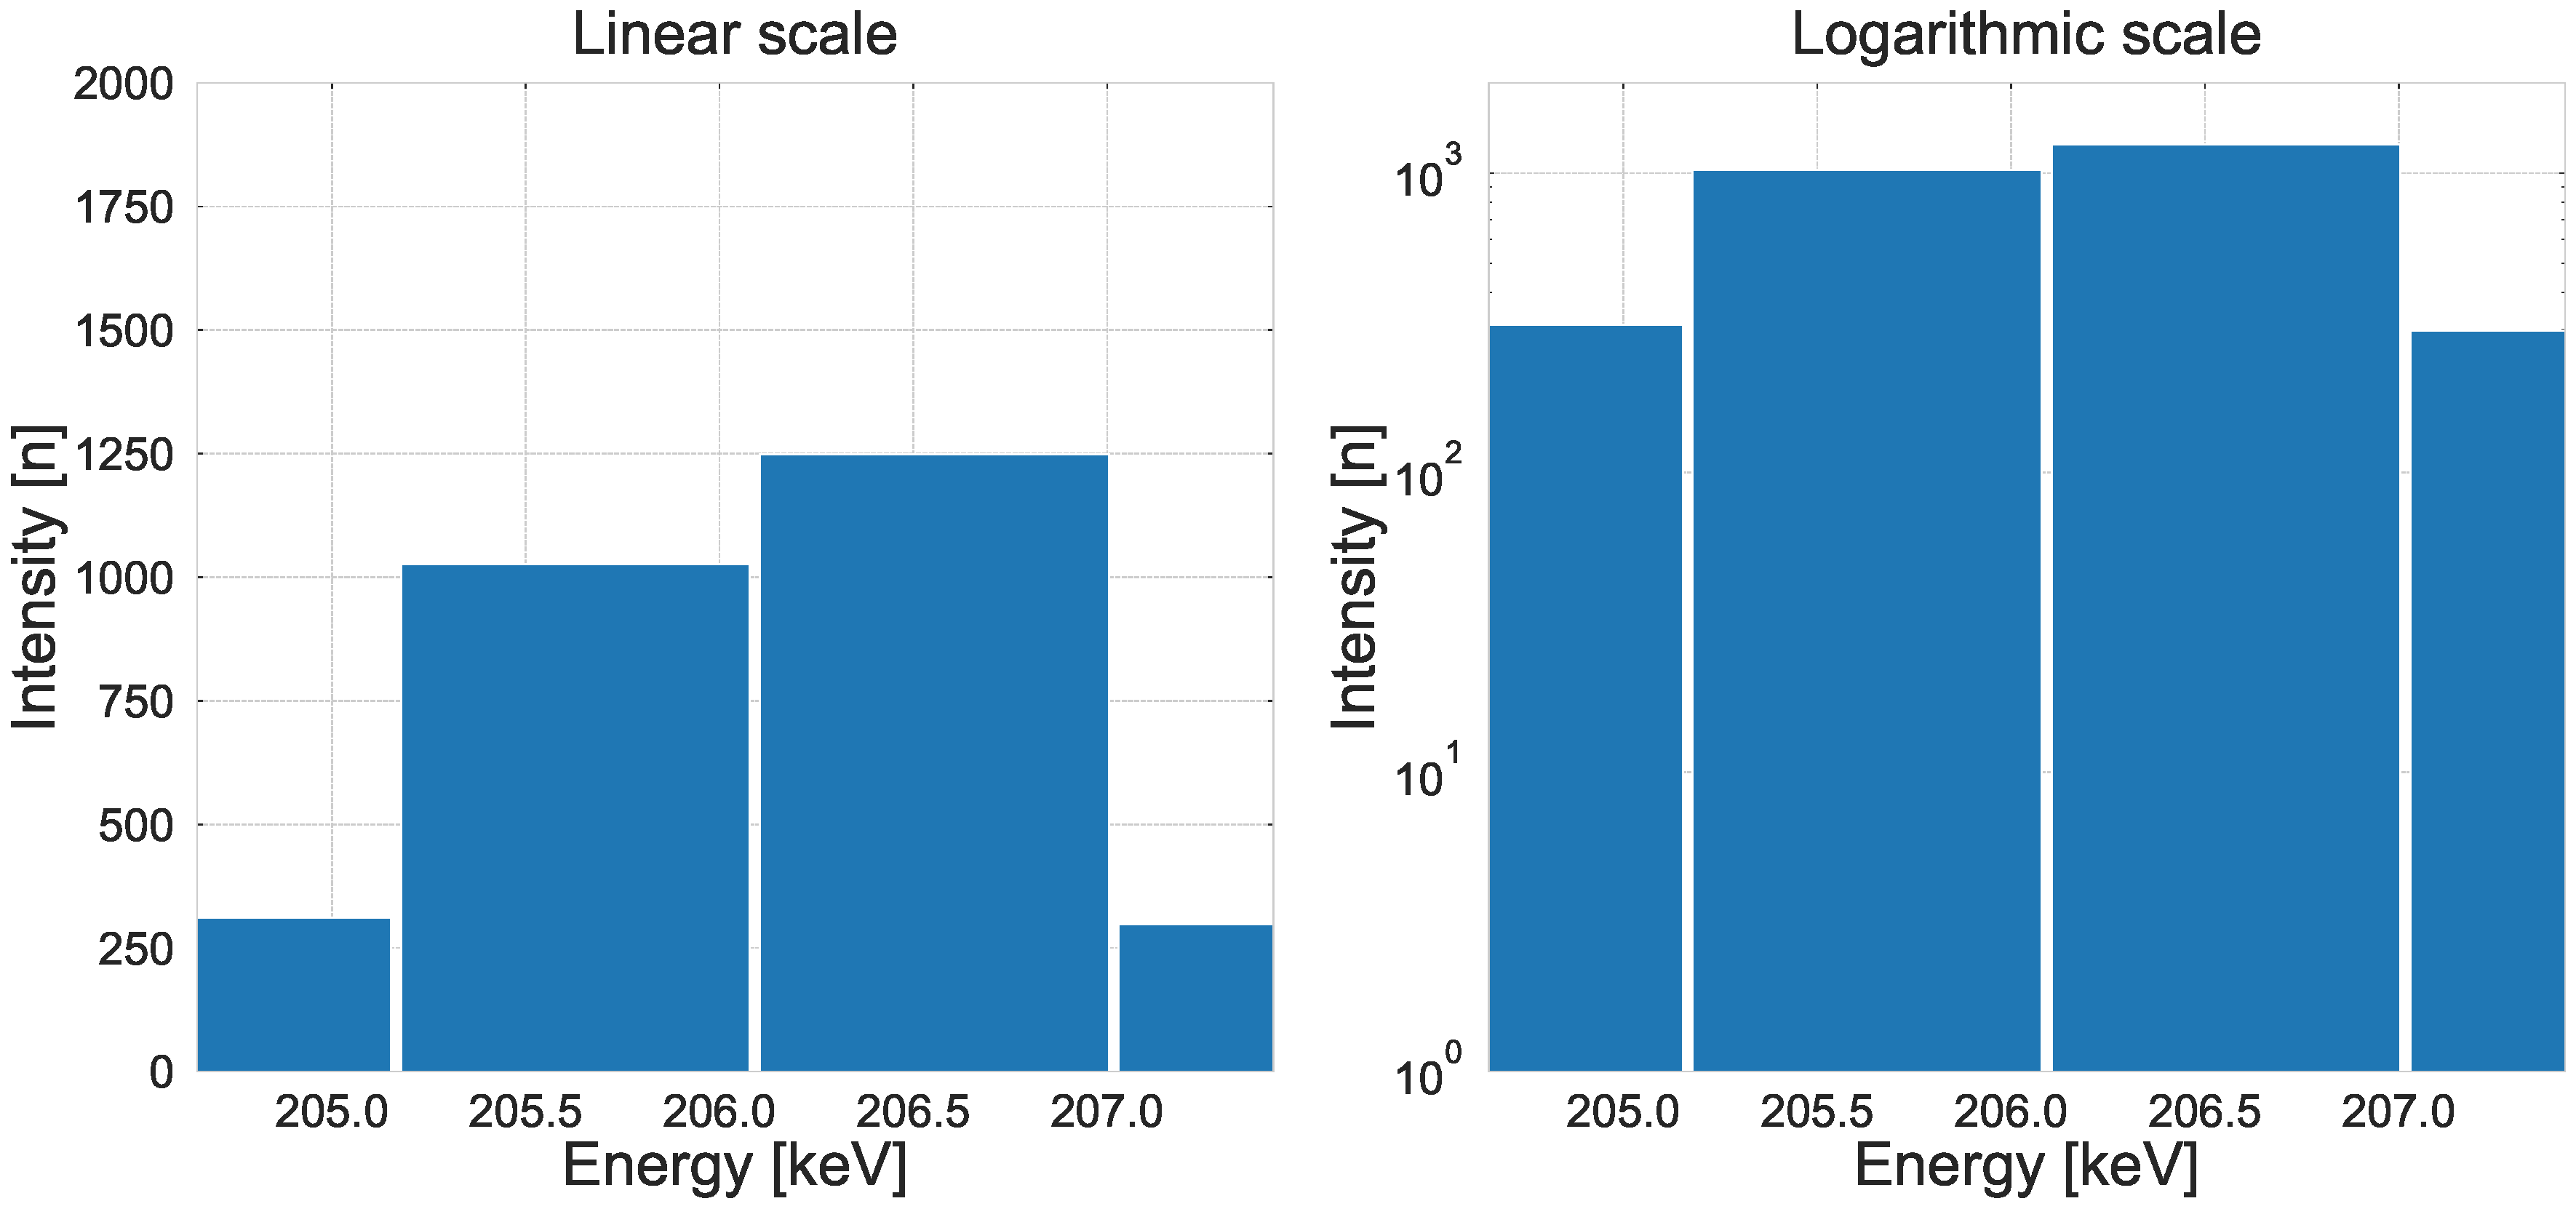
\includegraphics[width=\textwidth]{{images/spectra_lims_204.65_207.43_U235_g5_0}.pdf}
    \captionof{figure}{Az általam vizsgált anyag gamma-spektrumában található $^{235}$U, $\gamma_{5,0}$ tranziensből származó fotonjának foto-csúcsa.} \label{fig:7}
\end{center}
\begin{center}
    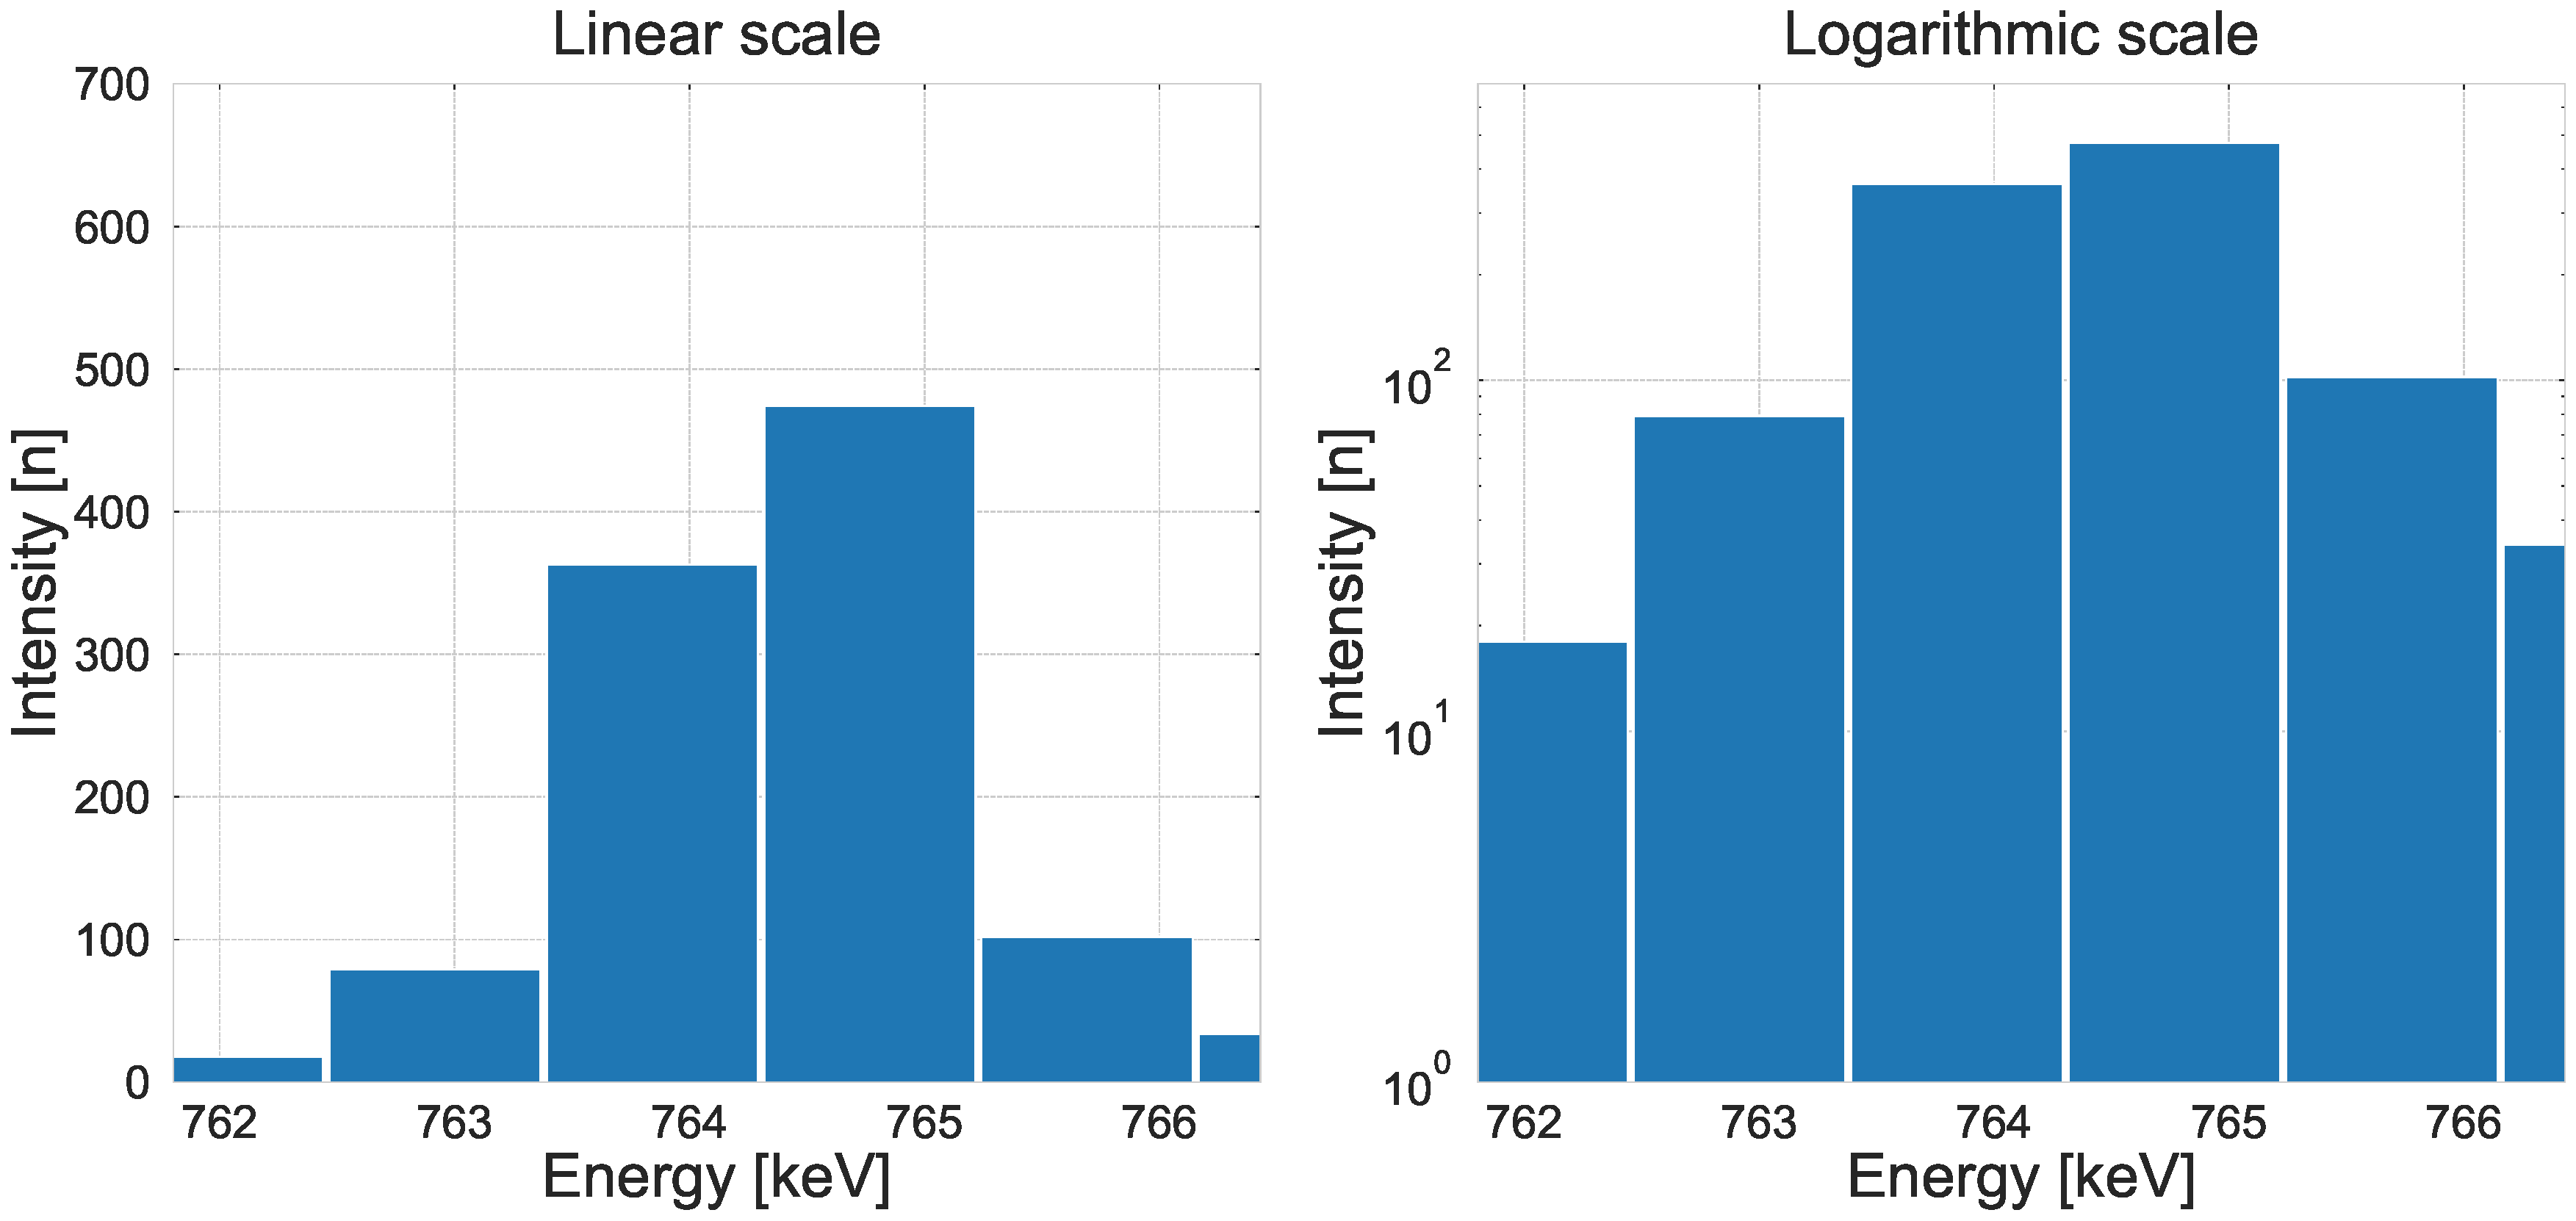
\includegraphics[width=\textwidth]{{images/spectra_lims_761.80_766.43_Pam234_g4_1}.pdf}
    \captionof{figure}{Az általam vizsgált anyag gamma-spektrumában található $^{234}$Pa$^{m}$, $\gamma_{4,1}$ tranziensből származó fotonjának foto-csúcsa.} \label{fig:8}
\end{center}
\begin{center}
    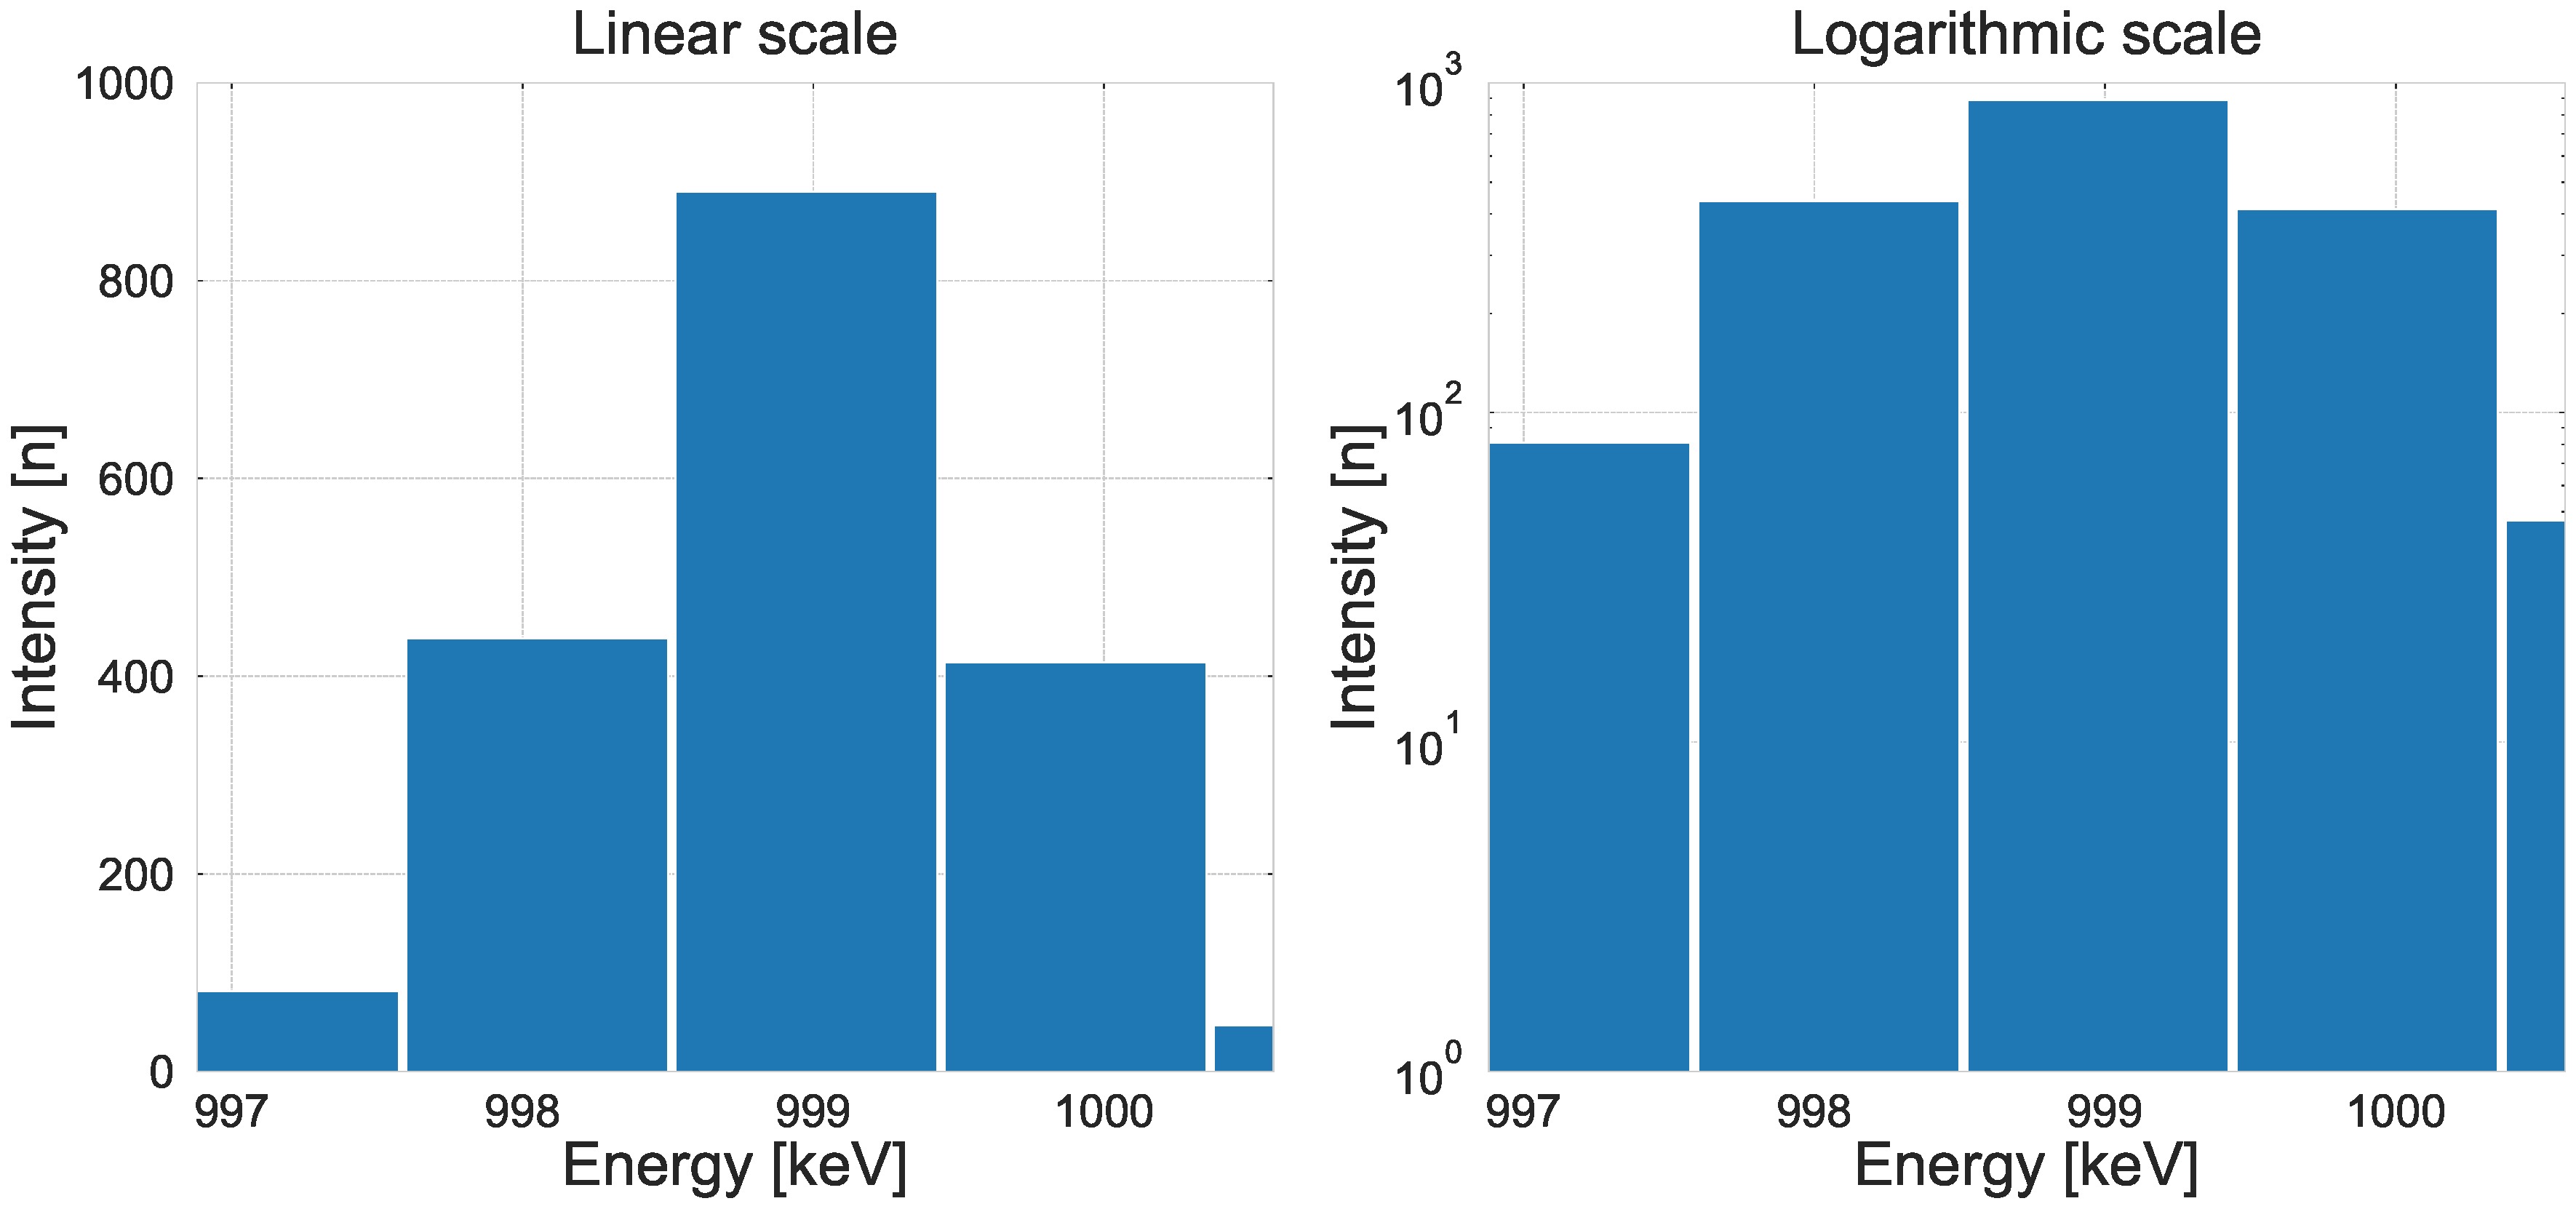
\includegraphics[width=\textwidth]{{images/spectra_lims_996.88_1000.58_Pam234_g9_1}.pdf}
    \captionof{figure}{Az általam vizsgált anyag gamma-spektrumában található $^{234}$Pa$^{m}$, $\gamma_{9,1}$ tranziensből származó fotonjának foto-csúcsa.} \label{fig:9}
\end{center}
\vspace*{\fill}

\section{ - Táblázatok} \label{appendix:C}
\begin{center}
\begin{tabular}{|c|c|c|c|c|c|c|}
\hline
Izotóp 			 & Mért $E_{\gamma}$ [keV] & Valós $E_{\gamma}$ [keV]  & Intenzitás [\%] & Tranziens             & $S_{\text{csúcs}}$ & $\delta S_{\text{csúcs}}$ [\%] \\
\hline
$^{235}$U        & $145,28$       & $143,768$       & $13,20$          & $\gamma_{\text{4,1}}$ & $3375$  & $2,35$ \\
$^{235}$U  		 & $164,75$ 	  & $163,358$       & $5,855$          & $\gamma_{\text{5,1}}$ & $1976$  & $4,05$ \\
$^{235}$U  	     & $186,79$ 	  & $185,722$       & $63,41$          & $\gamma_{\text{4,0}}$ & $20836$ & $0,73$ \\
$^{235}$U  		 & $206,10$ 	  & $205,316$       & $5,465$          & $\gamma_{\text{5,0}}$ & $1666$  & $2,86$ \\
$^{234}$Pa$^{m}$ & $764,24$ 	  & $766.708$       & $3,29 * 10^{-1}$ & $\gamma_{\text{4,1}}$ & $914$   & $3,75$ \\
$^{234}$Pa$^{m}$ & $998,77$ 	  & $1001,441$      & $8,56 * 10^{-1}$ & $\gamma_{\text{9,1}}$ & $1550$  & $2,16$ \\
\hline
\end{tabular}
\captionof{table}{A gamma-spektrum kiértékelésekor vizsgált csúcsok adatai, $t = 1073$ s mérési idő és $N = 264077$ db detektált jel után (\cite{lnhb_235U} és \cite{lnhb_234Pa_m}).} \label{table:1}
\end{center}

\begin{center}
\begin{tabular}{|c|c|c|c|}
\hline
Izotóp 			 & $E_{\gamma}$ [keV] & Intenzitás [\%] & Felezési idő \\
\hline
$^{243}$Cm       & $760$     & $0$              & $29,1$ év    \\
$^{249}$Cf       & $760$     & $2 * 10^{-2}$    & $351$ év     \\
$^{150}$Eu       & $762,03$  & $2,8 * 10^{-2}$  & $36.9$ év    \\
$^{239}$Pu       & $763,61$  & $2.22 * 10^{-8}$ & $24110$ év   \\
$^{241}$Am       & $763,9$   & $2 * 10^{-7}$    & $432.2$ év   \\
$^{110}$Ag$^{m}$ & $763,944$ & $22,14$          & $249.79$ nap \\
$^{152}$Eu       & $764,900$ & $2,15 * 10^{-1}$ & $	13.537$ év \\
$^{160}$Tb       & $765,28$  & $2,140$          & $72.3$ nap   \\
$^{252}$Es       & $765,30$  & $1,83 * 10^{-1}$ & $471.7$ nap  \\
$^{192}$Ir       & $765,8$   & $1,49 * 10^{-3}$ & $73.831$ nap \\
\hline
\end{tabular}
\captionof{table}{A $764.24$ keV-es csúcsot okozható, $50$ napnál hosszabb felezési idejű magok listája \citep{lnbl_nuclear}} \label{table:2}
\end{center}

\begin{center}
\begin{tabular}{|c|c|c|c|}
\hline
Izotóp 			 & Mért $E_{\gamma}$ [keV] & $\eta$ [\%]          & $\delta \eta$ [\%] \\
\hline
$^{235}$U 		 & $145,28$                & $1,33059 * 10^{-1}$  & $2,218$            \\
$^{235}$U 		 & $164,75$ 	           & $1,23267 * 10^{-1}$  & $2,336$            \\
$^{235}$U 		 & $186,79$ 	           & $1,00812 * 10^{-1}$  & $2,129$            \\
$^{235}$U        & $206,10$ 	           & $1,06556 * 10^{-1}$  & $3,085$            \\
$^{234}$Pa$^{m}$ & $764,24$ 	           & $2,1255 * 10^{-2}$   & $2,491$            \\
$^{234}$Pa$^{m}$ & $998,77$ 	           & $2,7098 * 10^{-2}$   & $2,365$            \\
\hline
\end{tabular}
\captionof{table}{A detektor $\eta$ hatásfoka az egyes foto-csúcsok energiatartományaiban} \label{table:3}
\end{center}

\begin{center}
\begin{tabular}{|c|c|c|c|c|c|c|}
\hline
Izotóp 			 & $A$ [Bq]  & $\Delta A$ [Bq] & $\delta A$ [\%] & $\lambda$ ($1/s$) & $N$ [db]         & $\delta N$ [\%] \\
\hline
$^{235}$U 		 & $179,1$   & $5,8$ 	       & $3,23$          & $3,12 * 10^{-17}$  & $5,74 * 10^{18}$ & $=\delta A$ \\
$^{235}$U 		 & $255,2$   & $11,9$ 		   & $4,68$          & $3,12 * 10^{-17}$  & $8,18 * 10^{18}$ & $=\delta A$ \\
$^{235}$U 		 & $287,4$   & $6,4$           & $2,25$          & $3,12 * 10^{-17}$  & $9,21 * 10^{18}$ & $=\delta A$ \\
$^{235}$U        & $281,8$   & $11,9$          & $4,20$          & $3,12 * 10^{-17}$  & $9,03 * 10^{18}$ & $=\delta A$ \\
$^{234}$Pa$^{m}$ & $9554,6$  & $430,1$         & $4,50$          & $4,92 * 10^{-18}$  & $1,94 * 10^{21}$ & $=\delta A$ \\
$^{234}$Pa$^{m}$ & $7939,6$  & $254,3$ 		   & $3,20$          & $4,92 * 10^{-18}$  & $1,61 * 10^{21}$ & $=\delta A$ \\
\hline
\end{tabular}
\captionof{table}{Az egyes foto-csúcsokhoz tartozó aktivitás értékek, bomlási állandók, valamit részecskeszámok és ezek hibái} \label{table:4}
\end{center}

\begin{center}
\begin{tabular}{|c|c|c|c|c|}
\hline
Pozíció & Mérés ideje [s]   & $N$ [db]   & $A$ [Bq]   & $\delta A$ [\%] \\
\hline
Nyitott & $100$             & $275$      & $2,75$     & $10$ \\
\hline
Zárt    & $601$             & $642$      & $1,07$     & $4$ \\
\hline
\end{tabular}
\captionof{table}{A háttérsugárzás mérése során kapott értékek} \label{table:5}
\end{center}